\documentclass{article}

\usepackage[margin=1in]{geometry}
\usepackage{wrapfig}
\usepackage{tkz-euclide}
\usepackage{csquotes}
\usepackage{hyperref}
\usepackage{graphicx}
\usepackage{siunitx}

\title{2021 Castro Valley Junior Math Tournament Problems}
\author{}
\date{}

\begin{document}
\maketitle

\section*{Mooving Cow}
Bessie the Cow is $5$ meters north of Farmer John's house.
She starts running east at $2$ meters per second.
After how many seconds will she be exactly $10$ meters away from Farmer John's house?
Express your answer in exact form.

\section*{Cowangle}
\begin{wrapfigure}{r}{0.35\linewidth}
	\vspace{-20pt}
	\centering
	\begin{tikzpicture}
		\tkzDefPoint(110:2){A}
		\tkzDefPoint(180:2){B}
		\tkzDefPoint(0:2){C}

		\tkzDefPointBy[projection=onto B--C](A)
		\tkzGetPoint{X}

		\tkzDrawPolygon(A,B,C)
		\tkzDrawSegment(A,X)
		\tkzLabelPoints[above](A)
		\tkzLabelPoints[left](B)
		\tkzLabelPoints[right](C)
		\tkzLabelPoints[below](X)
		\tkzMarkRightAngle(B,A,C)
		\tkzMarkRightAngle(A,X,C)
		\tkzLabelLine[above left](A,B){$7$}
		\tkzLabelLine[above right](A,C){$10$}
		\tkzLabelLine[right](A,X){?}
	\end{tikzpicture}
	\vspace{-20pt}
\end{wrapfigure}
Bessie the Cow found the following right triangle $ABC$.
The distance from point $A$ to point $B$ is $7$, and the distance from point $A$ to point $C$ is $10$.
$\angle A$ is a right angle, and $\overline{AX}$ is the altitude from point $A$ to side $\overline{BC}$.
What is the length of this altitude (the distance from point $A$ to point $X$)?
Express your answer in exact form.

\section*{Mooish}
Farmer Paul has two types of cows: truthy cows and falsy cows.
Physically, they are indistinguishable.
They all speak mooish, and they can be distinguished by how they answer questions.
The truthy cows always reply truthfully, and the falsy cows always lie.
Bessie had a conversation with three of Farmer Paul's cows: Annabelle, Betsie, and Cornelius.
Here's a translation of the conversation.
\begin{displayquote}
	Bessie: Annabelle, is Betsie truthy or falsy? \\
	Annabelle: Falsy \\
	Bessie: Betsie, are the types of Annabelle and Cornelius different? \\
	Betsie: No. \\
	Bessie: Talkative lot, aren't they? Cornelius, is Betsie truthy or falsy? \\
	Cornelius: Truthy.
\end{displayquote}
What is the type of each cow?

\section*{Green Cows}
Help Bessie the Cow answer the question ``How much grass can a green cow chow if green cows can chow grass?''
Bessie and Elsie both chow grass at constant rates.
If Bessie can chow all the grass in a field in $3$ hours and Elsie can chow all the grass in the same field in $4$ minutes, how long will it take for them to chow all the grass in this field together?
Express your answer in exact form.

\section*{My Cow Ate My Homework}
Bessie the Cow obtained Chloe's math homework again.
While she was enjoying this tasty snack, she noticed one problem that seemed very interesting.
Here's the problem statement:
\begin{displayquote}
	If two real numbers $a$ and $b$ are generate randomly and uniformly such that $-9 < a < 9$ and $-9 < b < 9$, what is the probability that $(a + b)^2 < 2ab + 9$?
	Express your answer in exact form.
\end{displayquote}
Bessie is bad at math, so help her by solving this problem.

\section*{Look Mom No Proof!}
Bessie the Cow found a website called \url{vixra.org} which mostly publishes scientific nonsense.
There's a paper (\url{https://vixra.org/abs/2008.0229}) which presents a simple method that supposedly checks whether integers greater than $5$ are prime.
It makes the following statement without proof:
\begin{displayquote}
    The answer to whether the given numbers are prime numbers is to check that:
    \begin{itemize}
        \item[a)] The numbers are not even numbers (the last digit is not divisible by $2$);
        \item[b)] The last digit of numbers in not $5$;
        \item[c)] The sum of the digits of each of the remaining numbers is not divisible by $3$.
    \end{itemize}
    A number that meets the above criteria is either a prime or a power [of a] prime.   
\end{displayquote}
Disprove this claim.

\section*{Mooshroom Pizza}
\begin{wrapfigure}{r}{0.35\linewidth}
	\vspace{-20pt}
	\centering
	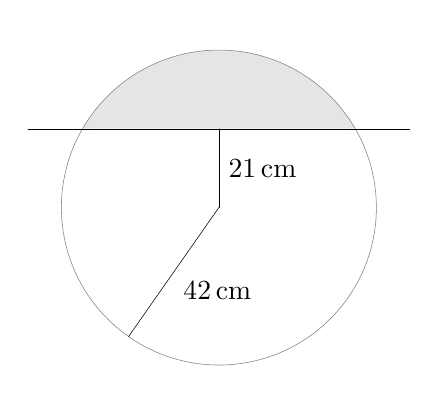
\begin{tikzpicture}[scale=0.5]
		\tkzDefPoint(0,0){A}
		\tkzDefPoint(0,4){B}
		\tkzDefPointBy[rotation=center A angle 60](B)
		\tkzGetPoint{C}
		\tkzDefPointBy[rotation=center A angle -60](B)
		\tkzGetPoint{D}
		\tkzFillSector[fill=gray!20](A,D)(C)
		\tkzDrawCircle(A,B)
		\tkzDrawPolygon[white,fill=white](A,C,D)
		\tkzDrawLine(C,D)
		\tkzDefMidPoint(C,D)
		\tkzGetPoint{E}
		\tkzDrawSegment(A,E)
		\tkzLabelSegment[right](A,E){$\SI{21}{cm}$}
		\tkzDefPointBy[rotation=center A angle 145](B)
		\tkzGetPoint{F}
		\tkzDrawSegment(A,F)
		\tkzLabelSegment[below right](A,F){\SI{42}{cm}}
	\end{tikzpicture}
	\vspace{-20pt}
\end{wrapfigure}
Farmer John made a mooshroom pizza for the cows.
(Mooshroom pizzas are ethically sourced and don't contain mooshroom meat.
They're called mooshroom pizzas because they contain mushrooms farmed from mooshrooms.)
Bessie tried to slice it, but she failed miserably, resulting in the cut shown in the following figure.
If the radius of the pizza is $\SI{42}{cm}$ cm and the cut is $\SI{21}{cm}$ cm away from the center of the pizza, what is the area of the smaller piece of pizza that was cut off?
Express your answer in exact form.

\section*{Cowcycles}
Bessie the Cow is participating in a bike race!
There are $5$ cows in the race, and they all bike at a constant speed on a circular track starting from the same position.
Bella takes $5$ minutes to complete one lap, Bessie takes $9$ minutes to complete one lap, Betty takes $3.5$ minutes to complete one lap, Betsie takes $9.8$ minutes to complete one lap, and Bossy takes $4.7$ minutes to complete one lap.
The cows have a weird tradition where once cow passes another after the race starts, they will instantaneously elbow bump each other.
In other words, each of the ${5 \choose 2} = 10$ possible pairs of cows will elbow bump each other any time they are in the exact same position after the start of the race.
For example, Bella and Bessie will elbow bump each other for the first time exactly $11.25$ minutes after the start of the race.
The cows race for $4$ hours.
How many elbow bumps will  occur in total?
Include any elbow bumps that occur exactly $4$ hours after the start of the race.

\section*{Cowtapult}
\begin{wrapfigure}{r}{0.35\linewidth}
    \vspace{-20pt}
    \centering
    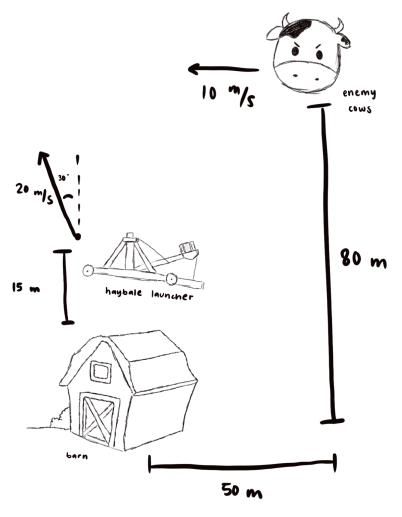
\includegraphics[scale=0.25]{cowtapult.png}
    \vspace{-20pt}
\end{wrapfigure}
Farmer Alex's barn is being attacked!!!!!
The enemy cows are in a cart that's currently $80$ meters north and $50$ meters east of the barn, and it is traveling west at $10$ meters per second.
Bessie the Cow is operating a cowtapult that is $15$ meters north of the barn.
The cowtapult launches a hay bale with a horizontal speed of $20$ meters per second in a direction that is $30$ degrees west from north.
Bessie wants to hit the enemy cart using the cowtapult.
When should she launch the hay bale?
Express your answer as a decimal in seconds, rounded to three digits after the decimal point.

\section*{Cowputing}
Bessie the Cow's new computing class has $N$ students.
If she kicks out $3$ students, she can split the students into groups of $8$.
If she adds $11$ students (to the original class of $N$ students), she can evenly split the students into groups of $5$.
If she adds $5$ students (to the original $N$ students), she can split the students into groups of $17$.
If she adds $1$ student, she can divide the students into $4$ groups each containing the same number of students.
What is the \textbf{second} smallest possible value of $N$?
\end{document}
